%\documentclass[11pt]{article}
\documentclass[11pt,a4paper]{tesis}
\usepackage[margin=1in]{geometry}          
\usepackage{graphicx}
\usepackage{amsthm, amsmath, amssymb}
\usepackage{setspace}\onehalfspacing
\usepackage[loose,nice]{units} %replace "nice" by "ugly" for units in upright fractions

\usepackage{hyperref}

 \begin{document}
\tableofcontents
\chapter{Introduction}
	\section{Problem description and motivation}
	\section{Objectives}
	\section{Previous work}
\chapter{Method}
	\section{Binary classification problem}
		(In Progress)

The task presented in this work is part of a broader set of problems: binary classification.
The main idea is to classify instances in two disjoint groups such as positives and negatives,
corrects and incorrects, true or false.

In this case, the objective is determining if different utterances were correctly or incorrectly 
pronounced. As it was said before, the chosen unit of anaylsis is the phone.

	\section{Features}
		\subsection{MFCC}
			\begin{itemize}
	\item Description. What are Mel Frequency Cepstral Coefficients?
	\item Normalization technique
	\item Motivation for varying window and shift
\end{itemize}
		\subsection{Gaussian Mixture Models}
			\begin{itemize}
	\item Gaussian Mixture Model
	\item Log Likelihood Ratio method to asses pronunciation
	\item GMM adaptation method
	\item Generating supervectors from adapted GMMs
\end{itemize}
		\subsection{Legendre polynomials}
			\begin{itemize}
	\item Definition and explanation of Legendre Polynomials
	\item Obtaining supervectors from Legendre Polynomials. Legendre coefficients
	\item Importance of fitting polynomial degree
\end{itemize}
			\subsubsection{Motivation}
				\begin{itemize}
	\item Modeling time dependencies
	\item Difference with Supervectors obtained from GMM adaptation
\end{itemize}
			\subsubsection{Regularization}
				\begin{itemize}
	\item Motivation of Regularization
	\item Ridge Regression
	\item Lasso Regression
\end{itemize}
	\section{Support Vector Machines}
		The chosen model for the discriminative analysis is the \textit{Support Vector Machine} classifier,
an approach for classification that was developed in the computer science community in the 1990s
and that has grown in popularity since then. The SVM is a member of the family of
\textit{maximal margin classifiers}, which base its strategy in finding the hyperplane that
best separate the positive and negative instances \cite{svm_jwht}.

\subsection{Maximal Margin Classifiers}
In a \textit{p-dimensional} space, a hyperplane is a flat affine subspace of
dimension $p-1$ defined by the equation:

\begin{equation}
  \label{eq:hyperplane}
  \beta_{0} + \beta_{1}X_{1} + \beta_{2}X_{2} + \dotsc + \beta_{p}X_{p} = 0
\end{equation}

The equation defines a \textit{p-dimensional} hyperplane in the sense that if a point
$X=(X_{1}, X_{2}, \dotsc, X_{p})^{T}$ in \textit{p-dimensional} space
satisfies \ref{eq:hyperplane} then $X$ lies on the hyperplane.

If $X$ doesn't lie in the hyperplane then either:

\begin{equation}
  \label{eq:hyperplaneGreater}
  \beta_{0} + \beta_{1}X_{1} + \beta_{2}X_{2} + \dotsc + \beta_{p}X_{p} > 0
\end{equation}

\begin{center}or\end{center}

\begin{equation}
  \label{eq:hyperplaneLesser}
  \beta_{0} + \beta_{1}X_{1} + \beta_{2}X_{2} + \dotsc + \beta_{p}X_{p} < 0
\end{equation}

So the hyperplane somehow divides the \textit{p-dimensional} space into two halves. One can
easily determine on which side of the hyperplane a point lies by simply calculating the sign
of the left hand side of \ref{eq:hyperplane}.

Having a set of $n$ instances of dimension $p$, with labels
$y_{1}, y_{2}, \dotsc y_{n} \in \{-1,1\}$ and $x^{i} = (x^{i}_{1}, x^{i}_{2}, \dotsc x^{i}_{p}) \ \forall \ 1 \leq i \leq {n}$ and supposing that it is possible to construct a hyperplane that
separates the training observations perfectly according to their class labels, then a
separating hyperplane has the property that:

\begin{equation}
\beta_{0} + \beta_{1}X_{1} + \beta_{2}X_{2} + \dotsc + \beta_{p}X_{p} > 0 \ if \ y_{i} = 1
\end{equation}

\begin{center}and\end{center}

\begin{equation}
\beta_{0} + \beta_{1}X_{1} + \beta_{2}X_{2} + \dotsc + \beta_{p}X_{p} < 0 \ if \ y_{i} = -1
\end{equation}

A test observation $x^{*}$ is classified based on the sign of
$f(x^{*})=\beta_{0}+\beta_{1}x^{*}_{1} + \beta_{2}x^{*}_{2} + \dotsc + \beta_{p}x^{*}_{p}$.
If $f(x^{*})$ is positive, then it is assigned to class 1 whereas if $f(x^{*})$ is negative
then it is assigned to class -1. In addition, the magnitude of $f(x^{*})$ also contains valuable
information.
If $f(x^{*})$ is far from zero then it means that $x^{*}$ lies far from the hyperplane
whereas if $f(x^{*})$ is close to zero then $x^{*}$ is located near the hyperplane and
there is less certainty about the class of $x^{*}$.

In general, if the data can be perfectly separated using a hyperplane, then there will be an
infinite number of such hyperplanes. This is because a given separating hyperplane can usually
be shift a tiny bit up or down, or rotating without coming into contact with any of the
observations.

\begin{figure}[H]
  \centering
  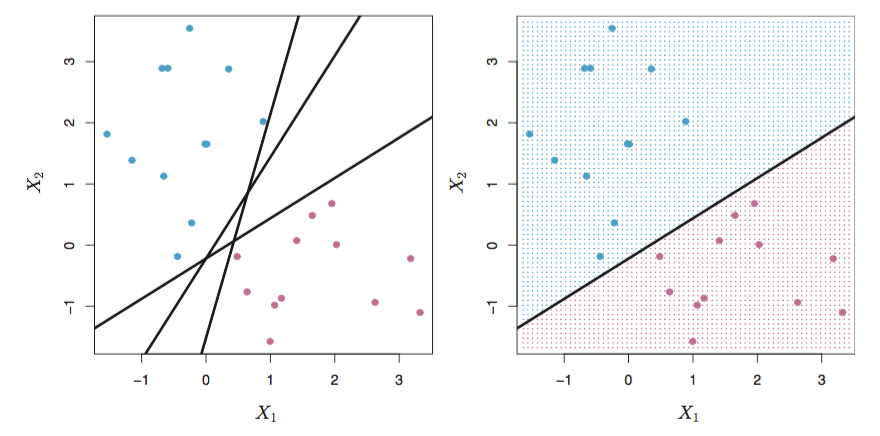
\includegraphics[width=0.8\textwidth]{files/figures/method/max-margin}
  \caption{Taken from \textit{JWHT} \cite{svm_jwht} book.
  Left: Three separating hyperplanes out of many
  possibilities. Right: Optimal Separating Hyperplane for the same dataset. A test observation
  that falls in the blue portion of the grid will be assigned to the blue class, and a test
  observation that falls in the purple portion of the grid will be assigned
  to the purple class.}
  \label{fig:maxMargin}
\end{figure}

A natural choice is the \textit{Maximal Margin Classifiers} (also known as the
\textit{Optimal Separating Hyerplane}), which is the separating hyperplane that is farthest
from the training observations. The \textit{margin} of the hyperplane is computed as the
minimal perpendicular distance to the hyperplane among all the training observations.
The maximal margin hyperplane is the separating hyperplane for which the margin is the largest.
The core idea is that a classifier that has a large margin on the training data will also
have a large margin on the test data.

\subsection{Support Vectors}

The separating hyperplane is determined by the instances of both classes that lies on the margin
of the hyperplane. These observations are known as \textit{Support Vectors}.
Observations can be interpreted as vectors in a \textit{p-dimensional} space and they
"support" the maximal
margin hyperplane in the sense that if these points were moved slightly then the maximal
margin hyperplane would move as well. The maximal margin hyperplane depends directly on the
support vectors, but not on the other observations: a movement to any of the other observations
would not affect the separating hyperplane, provided that the observation's movement does not cause
it to cross the boundary set by the margin.

\begin{figure}[H]
  \centering
  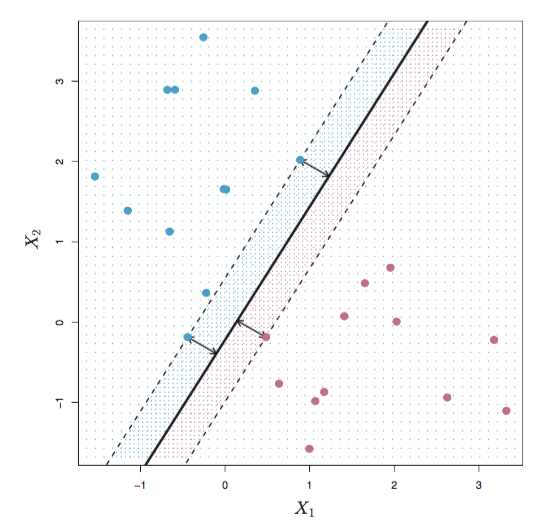
\includegraphics[width=0.4\textwidth]{files/figures/method/support-vectors}
  \caption{Taken from \textit{JWHT} \cite{svm_jwht} book. The maximal margin hyperplane
  is shown as a solid line. The margin is the distance between the solid line to either
  of the dashed lines. The two blue points and the purple point that line on the
  dashed lines are the support vectors.}
  \label{fig:maxMargin}
\end{figure}

\subsection{Problem Formulation}

It can be proven that given a set of $n$ observations of dimension $p$, the problem of
finding the \textit{Maximal Margin Hyperplane} can be posed as an optimization problem:
minimize $\| w \| = (\beta_{1}, \dotsc, \beta_{p})$.

\begin{equation}
\label{eq:svmOptimization}
w^{T}x^{*} = p\| w \|
\end{equation}

where $x^{*}$ is an observation and $p$ is the length of the projection of the observation
onto the normal vector of the hyperplane, i.e, the distance to the hyperplane.
Equation \ref{eq:svmOptimization} states that in order to maximize $p$ the norm of $w$
has to be minimized. On the other hand, the minimization problem is subject to the constraint:

\begin{equation}
  \label{eq:svmConstraint}
  y_{i} * (\beta_{0} + \beta_{1}x_{1} + \beta_{2}x_{2} + \dotsc + \beta_{p}x_{p}) > 0 \ \forall \ 1 \leq i \leq {n}
\end{equation}

Equation \ref{eq:svmConstraint} can be easily derived from \ref{eq:hyperplaneGreater} and
\ref{eq:hyperplaneLesser}.  This context matches the necessary conditions to apply
the \textit{Lagrange Multipliers} technique, to get this problem into a form
that can be solved analytically.

In practice, real data is scarcely ever completely linearly separable
and there is a trade off between
minimizing $\| w \|$ (i.e separating the instances by the largest possible margin)
and satisfying the constraint imposed over every
observation to lie on the right side of the hyperplane.
The desired hyperplane is one which separates correctly the vast majority of the observations and
at the same time it separates them by the largest margin. For this reason, when training an
\textit{SVM} classifier an additional parameter $C$ is passed as argument to the training
method in order to prioritize one problem over the other. A bigger $C$ favors the correctly
classification of the instances, while a smaller one favors the minimization of $\| w \|$
and thus finding the hyperplane with the largest margin for most of the instances.

(Agregar foto del efecto del parámetro C)

(Agregar la aclaración de que no vamos a comentar acerca de los kernels no lineales porque
no se usan)

		\subsection{Cost function}
			\begin{itemize}
	\item Formula: $C*\displaystyle\sum_{i=1}^{m} [y^{(i)} * cost_{1}(\theta^{T} * x^{(i)}) + (1-y^{(i)}) * cost_{0}(\theta^{T} * x^{(i)}))] + \frac{1}{2} * \displaystyle\sum_{j=1}^{n} \theta^{2}_{j}$
	\item Formula description. Least square term vs regularization term
\end{itemize}
		\subsection{C parameter}
			\begin{itemize}
	\item Explanation: How does it affect to the equation?
	\item Consequences of using a small $C$
	\item Consequences of using a large $C$
\end{itemize}
		\subsection{Balancing class weights}
			\begin{itemize}
	\item Behaviour and consecuences of classifier if no action is taken when dealing with unbalanced data
	\item Solution for unbalanced data problem
\end{itemize}
		\subsection{Features scaling}
			\begin{itemize}
	\item Technique description: Removing the mean and scaling every feature to unit variance
	\item Scaling effects from a max margin classification perspective
\end{itemize}
		\subsection{Feature combination}
			\begin{itemize}
	\item Training classifier from features of different sources
	\item Applying a correction factor to balance both features
\end{itemize}
	\section{Performance measures}
		\subsection{ROC Curve}
			\begin{itemize}
	\item Standard explanation of ROC curve
\end{itemize}
		\subsection{Equal error rate}
			In order to measure the performance of the different systems, the \textit{Equal Error Rate} metric
is chosen. As its name suggests, the \textit{EER} prioritizes in an equal manner the
\textcolor{red}{
  \textit{False Positive Rate} and the \textit{False Negative Rate}.
}
This metric was used
in the previous works of the current line of investigation related to pronunciation assessment
at phone level \cite{detection_phone_level_mispronunciation_learning, main}, so the same approach
was taken in the present work.

The process for evaluating the performance of a classifier usually involves the following steps:
At first, the decision function of the classifier, which can be for example predicted probabilities
or in our case distances to the hyperplane, is computed for each instance of the test set.
Then, the obtained results are used to generate
a distribution of the instances count as function of the values
in the domain of the decision function. Finally,
in order to make class predictions a threshold is chosen and the instances with a result of the
decision function above that threshold are classified as positive, while
those with results below the threshold are classified as negative. Most classifiers
usually set a threshold by default, such as 0 in the case of Support Vector Machines that
determines a separation of
positives and negative instances according to the sign of their distance to the hyperplane.

The EER can be found by sweeping the threshold until reaching the condition that
False Positive Rate (FPR) equals False Negative Rate (FNR). FPR is computed as
\textcolor{red}{the proportion} of negative instances wrongly
categorized as positive: $\frac{FP}{TN+FP}$.
Analogously, FNR is computed as \textcolor{red}{the proportion} of positve
instances wrongly categorized as negative:
$\frac{FN}{TP+FN}$. A simple example of EER threshold is
shown in Fig. \ref{fig:eer}.

\begin{figure}[H]
  \centering
  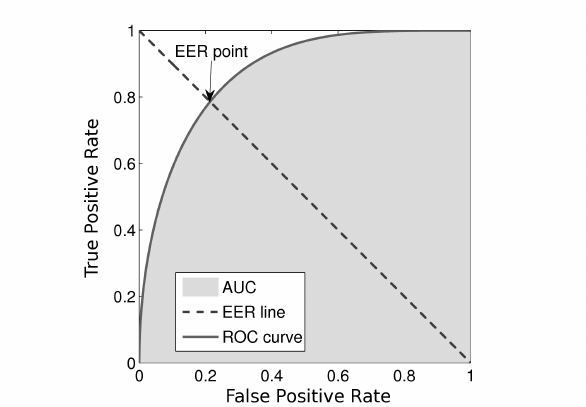
\includegraphics[width=0.8\textwidth]{files/figures/method/eer}
  \caption{An example of EER threshold with perfectly balanced classes. Both negative and positive distributions have the same size and shape.
  The threshold separates the instances in such way that FPR equals FNR.}
  \label{fig:eer}
\end{figure}

% Even though the diagram shows a case where the classes are perfectly balanced, in most of
% real world problems (including the current one) this does not happen. Distributions of both
% classes usually differs in both size and shape. However,
% as the technique is based on the \textit{rate} of misclassified positive and negative instances,
% the EER method can be applied without any trouble for unbalanced datasets and
% is computed exactly the same way: by sweeping the threshold until finding the point
% where FPR equals FNR.

\chapter{Experimental Design}
	\section{Speech Corpora}
		\subsection{Waveforms}
		\subsection{Alignments}
		\subsection{Labels}
	\section{Model training}
		\subsection{SVM from supervectors}
			\subsubsection{Balancing class weights}
			\subsubsection{Finding C parameter}
		\subsection{SVM from legendre coefficients}
			\subsubsection{Normalizing time axis}
			\subsubsection{Appending time durations}
			\subsubsection{Is duration by itself a good feature?}
			\subsubsection{Regularization: Finding best $\lambda$}
			\subsubsection{Best degree}
		\subsection{SVM from both sources}
			\subsubsection{Finding best proportion}

\chapter{Results}
	\section{Results on Development Set}
		\subsection{Results for SVM using supervectors}
		\subsection{Results for SVM using Legendre Coefficients}
		\subsection{Results for SVM using both sources}
	\section{Results on Held-out Data}
		\subsection{Results for SVM using supervectors}
		\subsection{Results for SVM using Legendre Coefficients}
		\subsection{Results for SVM using both sources}
\chapter{Conclusions}
 
\end{document}